\documentclass[12pt]{article}

% --- Packages ---
\usepackage[utf8]{inputenc}

\usepackage{hyperref}
\hypersetup{
    pdftitle= Bernoulli
}

\usepackage{amsmath, amssymb}
\usepackage{xcolor}
\usepackage{titlesec}
\usepackage{tcolorbox}
\usepackage{hyperref}
\usepackage[margin=1in]{geometry}
\usepackage{pgfplots}

\usepackage{parskip}

\usepackage{subcaption}  % Required for side-by-side subfigures

\usepackage{graphicx}
\usepackage{pgfplots} % Required for plotting
\pgfplotsset{compat=1.18} % Ensures consistent rendering across versions

% --- Custom Color Definitions ---
\definecolor{bgdark}{HTML}{1A1C20}     % Dark Background (#1A1C20)
\definecolor{emerald}{HTML}{2ECC71}    % Emerald Green Headers (#2ECC71)
\definecolor{purplehl}{HTML}{9B59B6}   % Purple Highlights (#9B59B6)
\definecolor{goldbox}{HTML}{F1C40F}    % Gold Formula Boxes (#F1C40F)
\definecolor{textlight}{HTML}{F8F9FA}  % Off-white text for dark background contrast

% --- Global Page Styling ---
\pagecolor{bgdark}
\color{textlight}

% --- Section & Subsection Styling ---
\titleformat{\section}{\color{emerald}\Large\bfseries}{\thesection}{1em}{}
\titleformat{\subsection}{\color{emerald}\large\bfseries}{\thesubsection}{1em}{}

% --- Custom Highlight & Formula Box Commands ---
\newcommand{\purplehighlight}[1]{\textcolor{purplehl}{\textbf{#1}}}

\newtcolorbox{goldformula}{
    colback=goldbox!10!bgdark, 
    colframe=goldbox,          % Gold border
    coltext=textlight,         % Light text inside box
    boxrule=1.5pt,
    arc=4pt,
    top=6pt,
    bottom=6pt
}

% --- Document Metadata ---
\title{\color{emerald}\Huge\bfseries The Bernoulli Distribution 
\author{\color{purplehl}Author: Muktadir Shihab}}

\begin{document}

\maketitle
\begin{figure}[htbp]
    \centering
    
    \begin{subfigure}[b]{0.45\textwidth} 
        \centering
        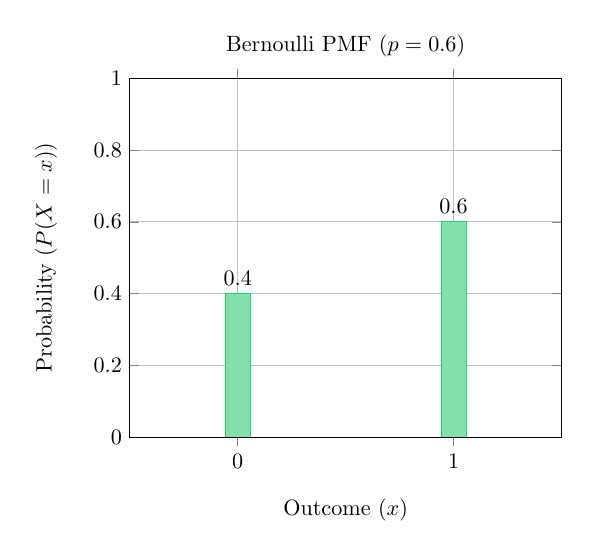
\begin{tikzpicture}[scale=0.8]
            \begin{axis}[
                ybar,
                ymin=0, ymax=1,
                xmin=-0.5, xmax=1.5,
                xtick={0,1},
                ytick={0, 0.2, 0.4, 0.6, 0.8, 1.0},
                xlabel={Outcome ($x$)},
                ylabel={Probability ($P(X=x)$)},
                xlabel style={at={(axis description cs:0.5,-0.15)}, anchor=north},
                ylabel style={at={(axis description cs:-0.15,0.5)}, anchor=south},
                nodes near coords,
                bar width=0.4cm,
                grid=major,
                title={Bernoulli PMF ($p = 0.6$)}
            ]
                \addplot[fill=emerald!60, draw=emerald] coordinates {(0,0.4) (1,0.6)};
            \end{axis}
        \end{tikzpicture}
        \caption{Discrete Bernoulli PMF.}
        \label{subfig:bernoulli_pmf}
    \end{subfigure}
    \hfill 
    \begin{subfigure}[b]{0.45\textwidth} 
        \centering
        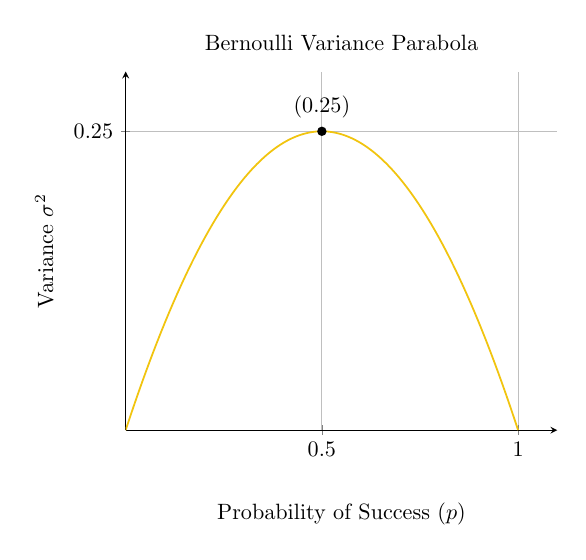
\begin{tikzpicture}[scale=0.8]
            \begin{axis}[
                axis lines = middle,
                xlabel={Probability of Success ($p$)},
                ylabel={Variance $\sigma^2$},
                xlabel style={at={(axis description cs:0.5,-0.18)}, anchor=north},
                ylabel style={at={(axis description cs:-0.15,0.5)}, anchor=south, rotate=90},
                xmin=0, xmax=1.1, 
                ymin=0, ymax=0.3,
                xtick={0, 0.5, 1},
                ytick={0, 0.25},
                grid=major,
                title={Bernoulli Variance Parabola}
            ]
                \addplot [
                    domain=0:1, 
                    samples=100, 
                    color=goldbox, 
                    thick
                ] {x*(1-x)};
                
                \node[label={90:{(0.25)}},circle,fill,inner sep=1.5pt] at (axis cs:0.5,0.25) {};
            \end{axis}
        \end{tikzpicture}
        \caption{Peaks at $p=0.5$.}
        \label{subfig:bernoulli_parabola}
    \end{subfigure}

    \caption{Probability Mass Function of Bernoulli Distribution vs. Bernoulli Perabola.}
\end{figure}

\newpage
\section{Introduction: The Atom of Uncertainty}
At the core of information theory and statistical mechanics sits the act of flipping a coin. While universally recognized as a symbol of pure randomness---a binary fork in the road where the universe splits between success and failure---it is also the fundamental building block of highly complex modern systems.

In statistical theory, this single binary event is formally defined as a \purplehighlight{Bernoulli Random Variable}, denoted as $X \in \{0, 1\}$. Its probability mass function is elegantly simple:
\begin{align*}
P(X = 1) &= p \\
P(X = 0) &= 1 - p
\end{align*}

This simple binary trial is the theoretical anchor for advanced machine intelligence. Whether an efficient algorithm is compressing massive video files or a neural network is weaving fluent prose, these frenetic complexities ultimately reduce to millions of individual Bernoulli decisions working in tandem. In modern Artificial Intelligence, the output layer of binary classification models operates entirely on this atomic principle.


\subsection{Expected Value \& Variance Definition}

\subsection*{Expected Value}

The \textbf{Expected Value} (or mean) of a random variable is the long-run average value of repetitions of the same experiment. It represents the center of mass of the probability distribution.

\paragraph{Definition:}
For a random variable $X$ defined on a probability space $(\Omega, \mathcal{F}, P)$, the expected value, denoted as $\mathbb{E}[X]$ or $\mu$, is the integral of $X$ with respect to the probability measure $P$:
\[
\mathbb{E}[X] = \int_{\Omega} X \, dP
\]

Depending on the nature of the random variable, this definition operationalizes into two primary mathematical forms:
\begin{itemize}
    \item \textbf{Discrete Random Variable:} If $X$ is a discrete random variable with a probability mass function (PMF) $p(x_i)$, the expected value is the weighted sum of all possible values:
    \[
    \mathbb{E}[X] = \sum_{i} x_i \cdot p(x_i)
    \]
    (Condition: The expected value exists if the sum is absolutely convergent, i.e., $\sum_{i} |x_i| p(x_i) < \infty$).
    
    \item \textbf{Continuous Random Variable:} If $X$ is a continuous random variable with a probability density function (PDF) $f(x)$, the expected value is the integral over the entire real line:
    \[
    \mathbb{E}[X] = \int_{-\infty}^{\infty} x \cdot f(x) \, dx
    \]
    (Condition: The expected value exists if $\int_{-\infty}^{\infty} |x| f(x) \, dx < \infty$).
\end{itemize}

\subection*{Variance}

The \textbf{Variance} measures the dispersion or spread of a random variable around its expected value. It quantifies how much the values of the random variable fluctuate from the mean.

\paragraph{Definition:}
Let $X$ be a random variable with a finite expected value $\mu = \mathbb{E}[X]$. The variance of $X$, denoted as $\text{Var}(X)$ or $\sigma^2$, is defined as the expected value of the squared deviation of $X$ from its mean $\mu$:
\[
\text{Var}(X) = \mathbb{E}\left[(X - \mathbb{E}[X])^2\right]
\]

Using the linearity of expectation, this definition is frequently simplified computationally to the identity:
\[
\text{Var}(X) = \mathbb{E}[X^2] - (\mathbb{E}[X])^2
\]

\begin{itemize}
    \item \textbf{Discrete Random Variable Form:}
    \[
    \text{Var}(X) = \sum_{i} (x_i - \mu)^2 \cdot p(x_i)
    \]
    
    \item \textbf{Continuous Random Variable Form:}
    \[
    \text{Var}(X) = \int_{-\infty}^{\infty} (x - \mu)^2 \cdot f(x) \, dx
    \]
\end{itemize}

\subsection*{Fundamental Differences}
\begin{itemize}
    \item \textbf{Dimensional Units:} If $X$ is measured in meters, the Expected Value $\mathbb{E}[X]$ is in meters, while the Variance $\text{Var}(X)$ is in meters squared ($\text{m}^2$). To revert to the original unit for dispersion, scientists take the square root of variance, known as the \textbf{Standard Deviation} ($\sigma = \sqrt{\text{Var}(X)}$).
    
    \item \textbf{Linearity:} Expected value is a linear operator:
    \[
    \mathbb{E}[aX + b] = a\mathbb{E}[X] + b
    \]
    Variance is not linear; scaling the variable squares the scale factor:
    \[
    \text{Var}(aX + b) = a^2\text{Var}(X)
    \]
\end{itemize}

\newpage

\section{Conceptual Framework: Physical Geometry \& Symmetry}
The standard formulas of statistics are frequently viewed as arbitrary rules, but they are in fact the inevitable geometric consequence of finding physical balance.

\subsection{The Expected Value as a Centroid}
Consider treating the abstract probabilities $p$ and $(1-p)$ as actual physical matter resting on a weightless rod. The Expected Value, $E[X]$, answers a simple physical question: where must a fulcrum be placed so that the system sits in perfect equilibrium?

\begin{goldformula}
\begin{equation}
E[X] = \sum_{x} x \cdot P(x) = 1(p) + 0(1 - p) = p
\end{equation}
\end{goldformula}

If a coin is fair ($p = 0.5$), the rod balances perfectly in the middle. If the system is heavily biased toward success (e.g., $p = 0.9$), the physical mass concentrates, and the fulcrum must glide smoothly to the right, landing precisely under the $0.9$ coordinate to maintain stability. The mathematical expected value is, quite literally, the \purplehighlight{physical center of gravity}.

\subsection{Variance as Rotational Inertia}
While the expected value locates the pivot, the variance dictates how the system behaves when spun. In statistics, variance measures the spread of possible outcomes. Physically, this is directly analogous to \purplehighlight{rotational inertia}---how much effort is required to spin the balanced rod.

\begin{goldformula}
\begin{equation}
\text{Var}(X) = E[(X - \mu)^2] = p(1 - p)
\end{equation}
\end{goldformula}

\paragraph{\purplehighlight{The Zone of Maximum Chaos:}}
When a coin is perfectly fair ($p = 0.5$), the masses are equal and distributed evenly around the center pivot. High inertia in the physical system corresponds directly to high variance ($0.25$). This point marks the absolute peak of the variance parabola, establishing 50/50 odds not as a safe bet, but as the mathematical \purplehighlight{zone of maximum chaos} and unpredictability.

Conversely, with a loaded coin (e.g., $p = 0.9$), almost all physical mass is concentrated directly on top of the pivot point. Spinning the rod becomes incredibly easy, and the variance shrinks to $0.09$. The outcome is highly predictable.

\section{Scaling the System: From Bernoulli to Binomial}
While an isolated Bernoulli trial models a single coin flip, real-world systems chain these events together. As trials are repeated, a branching tree of possible futures explodes exponentially, forming a physical pegboard of probability known as a \purplehighlight{Galton board}.

Each peg on a Galton board represents one independent Bernoulli trial. When thousands of these decisions occur simultaneously, the chaotic individual paths stack up into a remarkably predictable shape: the \purplehighlight{Binomial Distribution}, $B(n, p)$. Because expectation and variance are strictly additive for independent events, the center and spread of this complex macroeconomic shape are completely determined by the geometry of our single microscopic coin flip \cite{feller1968}.

\section{Modern Applications in Machine Learning}
The transition from visual, geometric metaphors to formal statistical theory seamlessly bridges into modern machine learning architectures \cite{goodfellow2016}. Tech giants and data scientists stack millions of Bernoulli variables to build sophisticated digital infrastructure.

\begin{itemize}
    \item \purplehighlight{Logistic Regression \& Sigmoid Activation:} The foundation of binary classification relies on the Sigmoid function, which dynamically outputs a $p$-value bounded between $0$ and $1$, explicitly defining the parameter for a Bernoulli distribution.
    \item \purplehighlight{A/B Testing \& Hypothesis Validation:} Whenever a user interacts with a platform (e.g., clicking a button yields a $1$, ignoring it yields a $0$), the interaction is a pure Bernoulli trial. Tech companies aggregate these trials to determine which interface version yields a higher expected value.
    \item \purplehighlight{Binary Cross-Entropy Loss:} The standard loss function utilized to train neural networks is derived directly from the Bernoulli likelihood function. By maximizing the likelihood of the observed binary data, the AI ``learns'' to adjust its weights.
\end{itemize}

\section{The Paradox of Predictability}
A common statistical trap is assuming that symmetric odds ($50/50$) offer safety. Mathematically, the exact opposite is true. To a statistician, \purplehighlight{predictability is safety}. Whether an outcome is a guaranteed success or a guaranteed failure, the variance approaches zero, and the ``rotational resistance'' of the mathematical system stabilizes \cite{shannon1948}.

By minimizing variance through massive datasets and complex modeling, modern AI systems essentially tighten the physical system around the fulcrum. Ultimately, mastering the statistical mechanics underlying these technologies does not require rote memorization of complex formulas; it requires building a rock-solid visual intuition for how systems naturally balance in geometric space.

% --- Cited References Section ---
\renewcommand{\refname}{\color{emerald} Cited References}
\begin{thebibliography}{9}

\bibitem{shannon1948}
Claude E. Shannon, \textit{A Mathematical Theory of Communication}, Bell System Technical Journal, vol. 27, pp. 379--423, 1948.

\bibitem{goodfellow2016}
Ian Goodfellow, Yoshua Bengio, and Aaron Courville, \textit{Deep Learning}, MIT Press, 2016.

\bibitem{feller1968}
William Feller, \textit{An Introduction to Probability Theory and Its Applications}, Vol. 1, 3rd Edition, John Wiley \& Sons, 1968.

\end{thebibliography}

\end{document}
